\documentclass[a4paper,12pt]{article}

\usepackage{graphicx}
\usepackage{float}
\usepackage[utf8]{inputenc}
\usepackage{booktabs}     % bảng đẹp
\usepackage{siunitx}      % căn số thập phân
\usepackage{geometry}
\geometry{margin=2.5cm}
\documentclass{article}
\usepackage[utf8]{inputenc}


\sisetup{
    table-format=2.2,
    round-mode=places,
    round-precision=2
}



\title{Report 2 - Gradient Descent}
\author{Le Nghiem Thanh Thuy}
\date{May 2026}

\begin{document}

\maketitle
\section{Algorithm}
This algorithm uses gradient descent to build a linear regression model for specified dataset
.
Here the result with initial value [0, 1] and learning rate 0.001
Model converges after ~17.000 epochs.




\begin{figure}[htbp] % [htbp] giúp định vị ảnh: here, top, bottom, page
    \centering % Câu lệnh căn giữa ảnh
    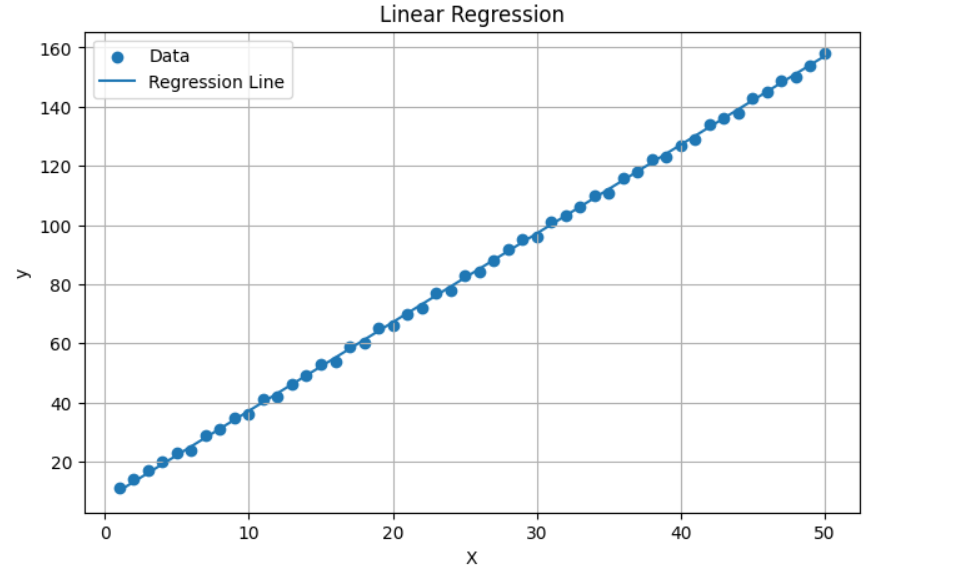
\includegraphics[width=0.5\textwidth]{LR_Result_2.png} % Điều chỉnh chiều rộng
    \caption{Result of model}
    \label{fig:my_label}
\end{figure}




\section{Loss}


\begin{figure}[htbp] % [htbp] giúp định vị ảnh: here, top, bottom, page
    \centering % Câu lệnh căn giữa ảnh
    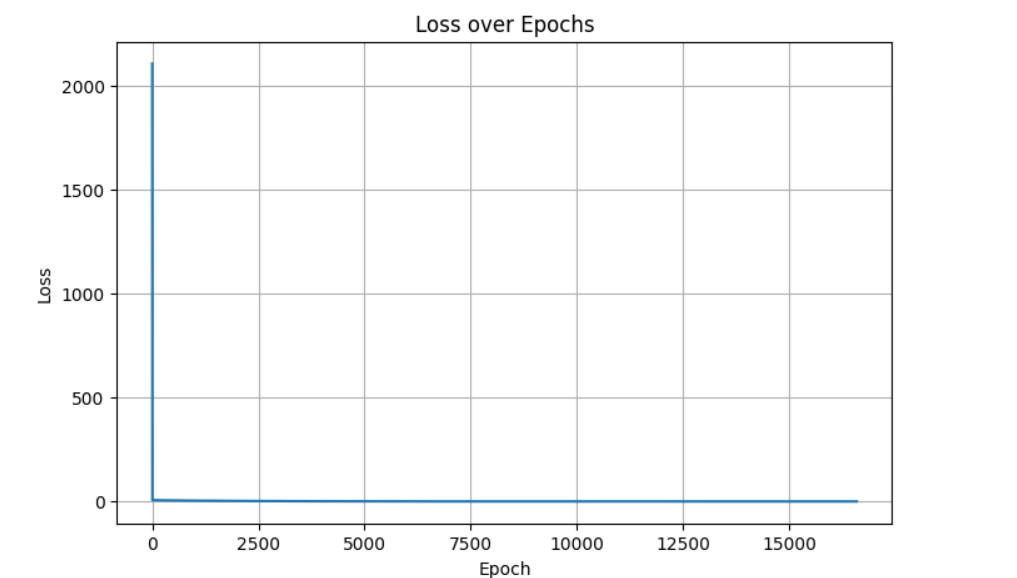
\includegraphics[width=0.5\textwidth]{LR_Loss_2.png} % Điều chỉnh chiều rộng
    \caption{Loss of model over epochs}
    \label{fig:my_label}
\end{figure}

\end{document}